\chapter{Algoritmos completos}

\section{Obtención de las celdas base}\label{algComp:celdasbase}
El algoritmo \ref{alg:celdasBaseCompleto} consiste en una version sin las
simplificaciones comentadas en la sección \ref{subsec:critPer} del algoritmo
\ref{alg:celdasBase}.

\begin{algorithm}[H]
\SetAlgoLined
  \SetKwInOut{Input}{Entrada}
  \Input{$c$}

% En updateBase c es pN y cA es p
% En setPseudoSourcesFromWave c es p y cA es waveP
  % \tcp{DFS desde $c$ agregando las celdas visitadas a la componente conexa $C_i$}
  $\mli{CB}_c := \emptyset$

  \ForEach{ $cA \in ady(c)$} {
    \ForEach{$b \in gens(cA)$} {
      $\mli{tolerado}  := d_c(b) - \mli{DD}(c) \leq L$\\
      % $\mli{noIgNiAdy} := b \notin gens(c) \land b \notin \bigcup_{b'} ady(gen(c))$\\

      $\mli{masCercano} := Verdadero$\\
      $\mli{aRemover} := \emptyset$\\
      \ForEach{$b' \in \mli{CB}_c$} {
        \If{$b' = b \lor b' \in ady(b)$}{
          \uIf{$d_c(b) < d_c(b')$}{
            $\mli{aRemover} := \mli{aRemover} \cup \{b'\}$\\
          }\Else{
            $\mli{masCercano} := \mli{masCercano} \land Falso$ \\
            \tcp{Se puede terminar de iterar una vez ejecutada esta línea}
          }
        }
      }
      
      \If{tolerado $\land$ masCercano}{
        $\mli{CB}_c := \mli{CB}_c -\mli{aRemover}$\\
        $\mli{CB}_c := \mli{CB}_c \cup \{\mli{b}\}$\\
      }
    }
  }
  \Return $\mli{CB}_c$ 

  \caption{Obtención de las celdas base $\mli{CB}_c$ de la celda $c$}
  \label{alg:celdasBaseCompleto}
\end{algorithm}

\newpage
Uno de los cambios principales es el remplazo de la función $gen$ por la
función $gens : \mli{CG} \rightarrow P(\mli{CGen})$ que dada una celda $c$ de
la grilla devuelve el conjunto de todas las celdas a mínima distancia de $c$ que pertenecen a
un generador. Otro cambio a notar es que la condición que en algoritmo
simplificado es controlada explícitamente con la variable $\mli{noIgNiAdy}$, en
este algoritmo completo se maneja implícitamente en la condición controlada
a través de la variable $\mli{masCercano}$. El ultimo cambio a destacar es que la
condición asociada a la variable $\mli{masCercano}$ (líneas 5-15) pasa a
ser que la celda base candidato $b$ esté a menor distancia de $c$ que las
celdas base actuales $b'$ de $c$ que son iguales o adyacentes a $b$, de cumplirse esta
condición dichos $b'$ dejan de ser celdas base de $c$.
\newpage

\chapter{Ejemplos completos}
\begingroup
\small
\section{Simplificación de fronteras basada en cubrimiento}\label{EXE:sfbc}
La figura \ref{EXE:sfbc} presenta la version completa del ejemplo mostrado en la figura \ref{fig:ejemploFSCub}.
\endgroup
\begin{figure}[H]
  \centerfloat
  \subfloat[Estado inicial.]{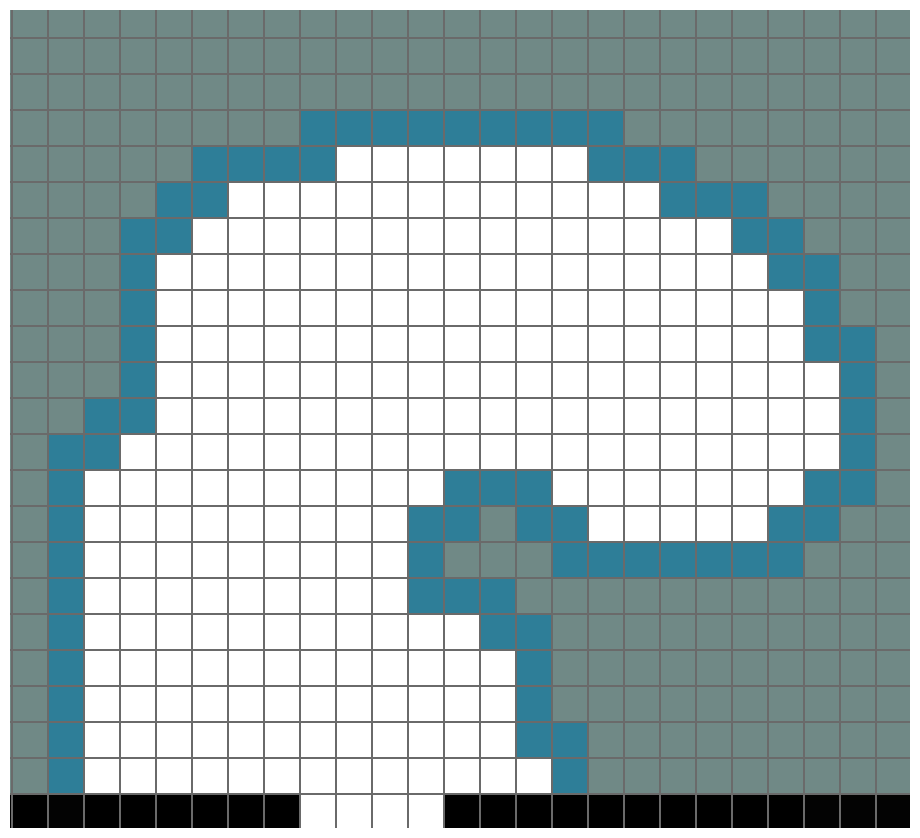
\includegraphics[clip=true, width=0.48\textwidth]{imagenes/ejemploSimpCub/a1.png}}
  \subfloat[Se inicializa $\mli{FP}$.]{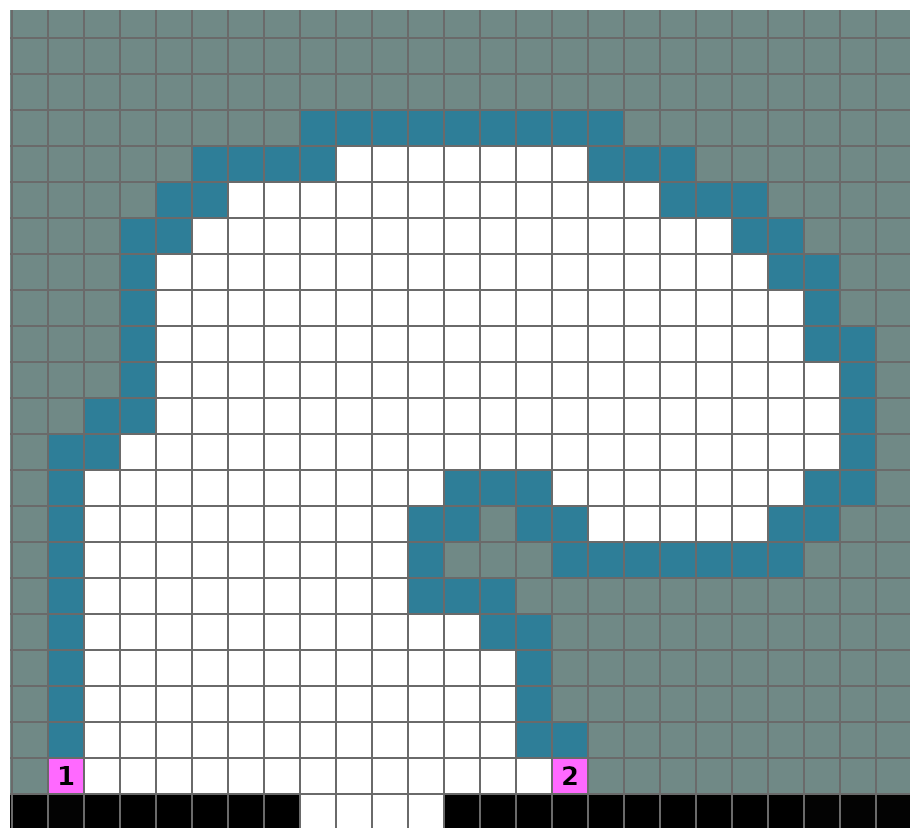
\includegraphics[clip=true, width=0.48\textwidth]{imagenes/ejemploSimpCub/a2.png}}

  \subfloat[Se obtiene $\mli{fp}$ desencolando de $\mli{FP}$.]{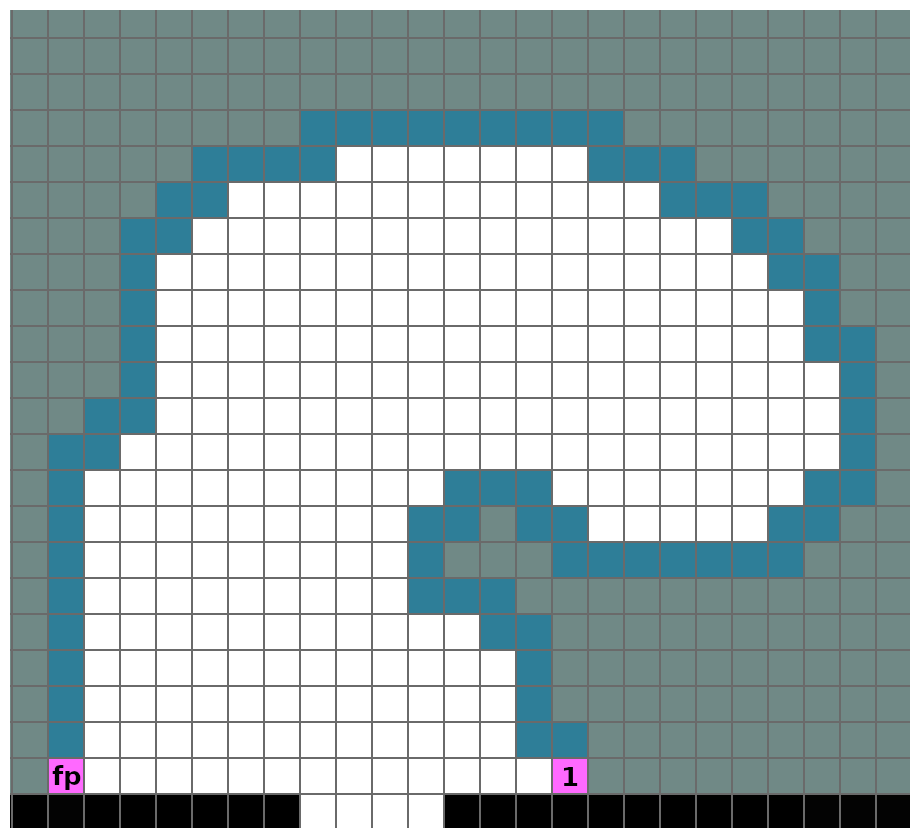
\includegraphics[clip=true, width=0.38\textwidth]{imagenes/ejemploSimpCub/b1.png}}
  \subfloat[Existen celdas más alejadas que $2*rango$, los candidatos se obtienen con $radio=rango$. ]{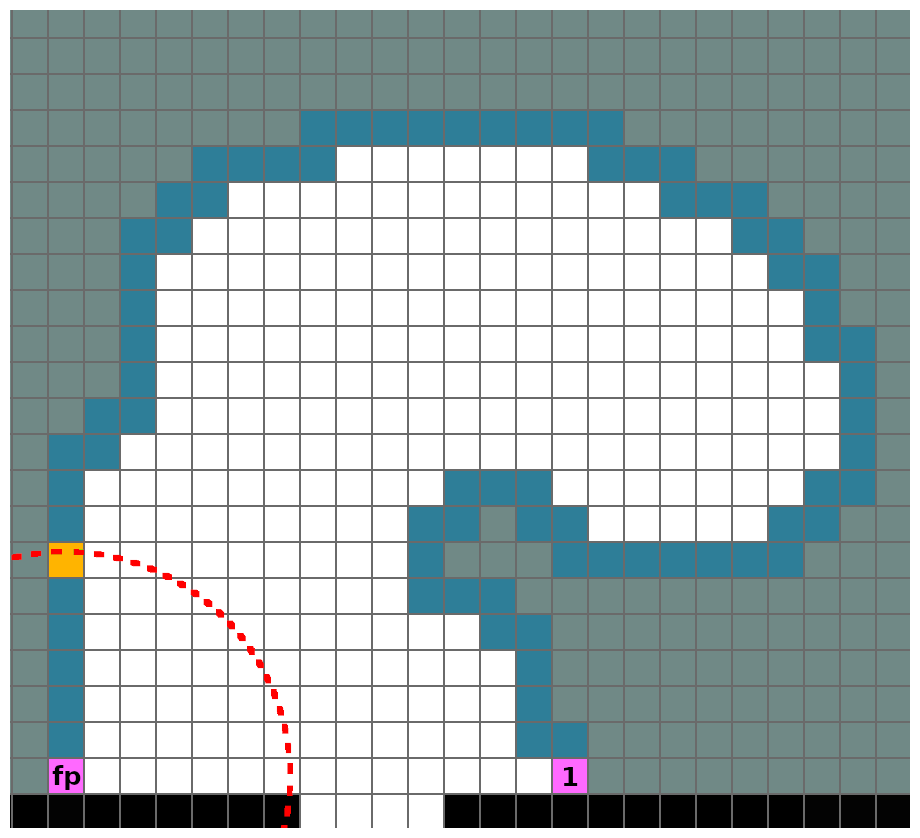
\includegraphics[clip=true, width=0.38\textwidth]{imagenes/ejemploSimpCub/b3.png}}
  \subfloat[Se elige el único candidato como $\mli{fs}$, se actualiza $\mli{UF}$, $\mli{FS_i}$ y $\mli{FP}$.]{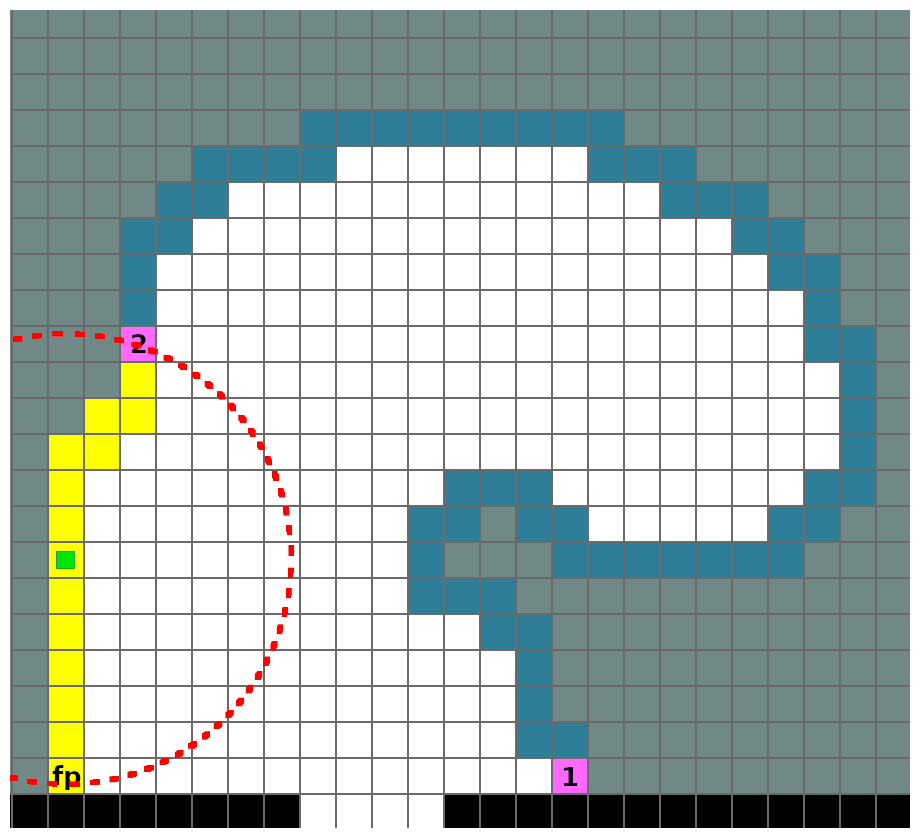
\includegraphics[clip=true, width=0.38\textwidth]{imagenes/ejemploSimpCub/b5.png}}

 \phantomcaption

\end{figure}

\begin{figure}[H]
  \setcounter{subfigure}{5}
  \centerfloat

  \subfloat[Se obtiene $\mli{fp}$ desencolando de $\mli{FP}$.]{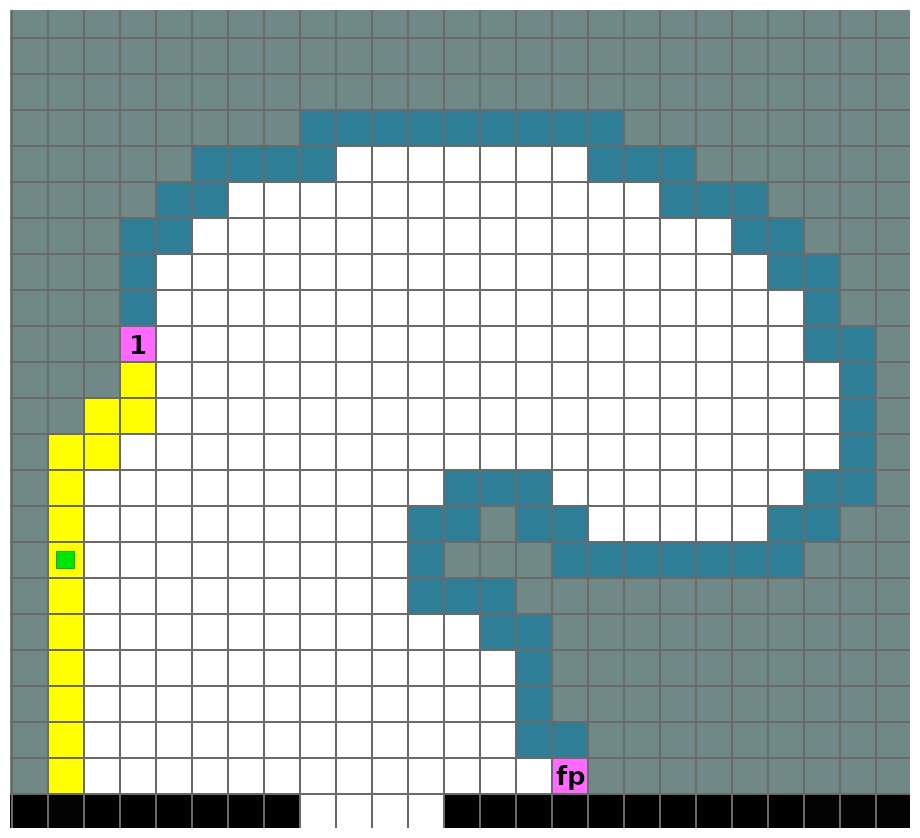
\includegraphics[clip=true, width=0.40\textwidth]{imagenes/ejemploSimpCub/c1.png}}
  \subfloat[Existen celdas más alejadas que $rango$, los candidatos se obtienen con $radio=rango$. ]{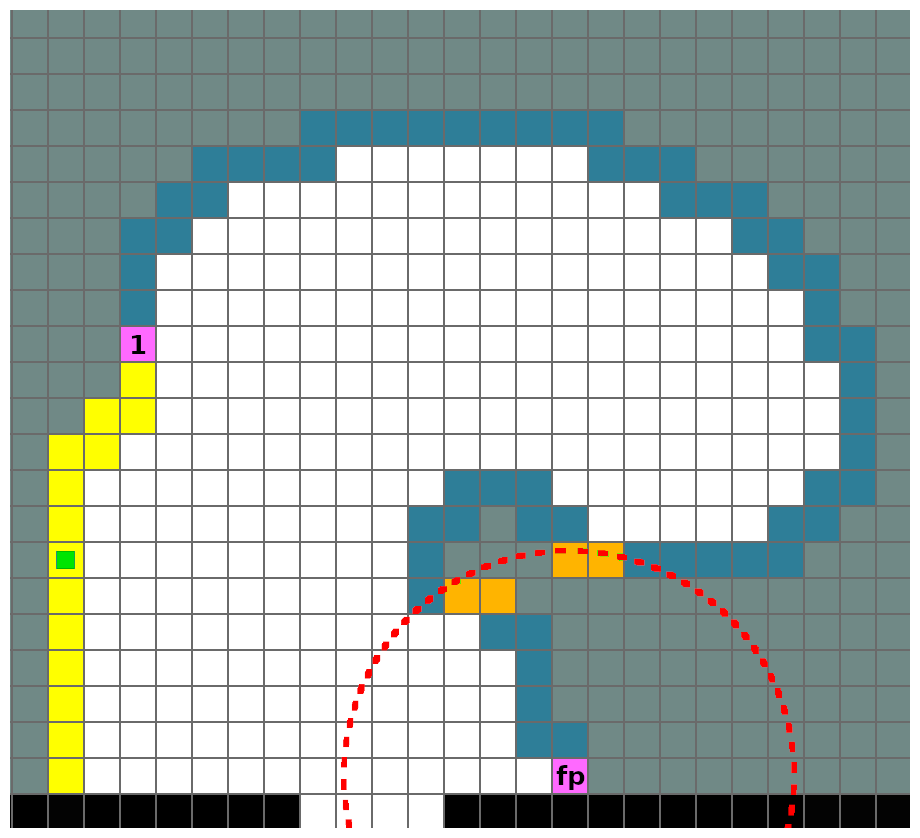
\includegraphics[clip=true, width=0.40\textwidth]{imagenes/ejemploSimpCub/c3.png}}
  \subfloat[Se elige arbitrariamente un candidato como $\mli{fs}$, se actualiza $\mli{UF}$, $\mli{FS_i}$ y $\mli{FP}$.]{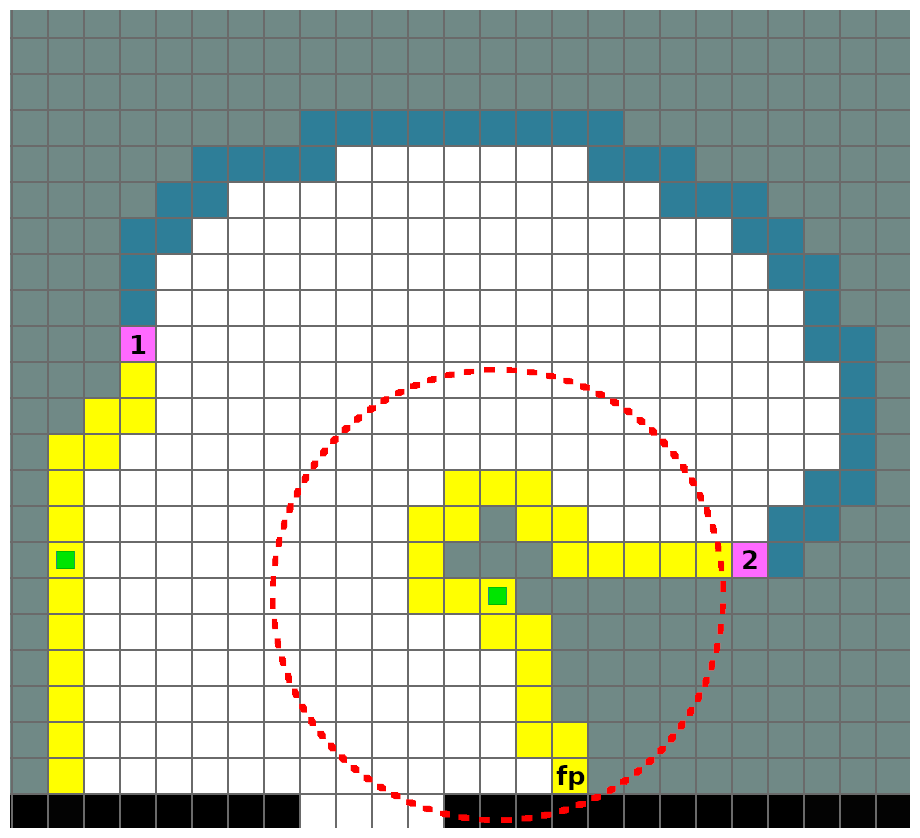
\includegraphics[clip=true, width=0.40\textwidth]{imagenes/ejemploSimpCub/c5.png}}


  \subfloat[Se obtiene $\mli{fp}$ desencolando de $\mli{FP}$.]{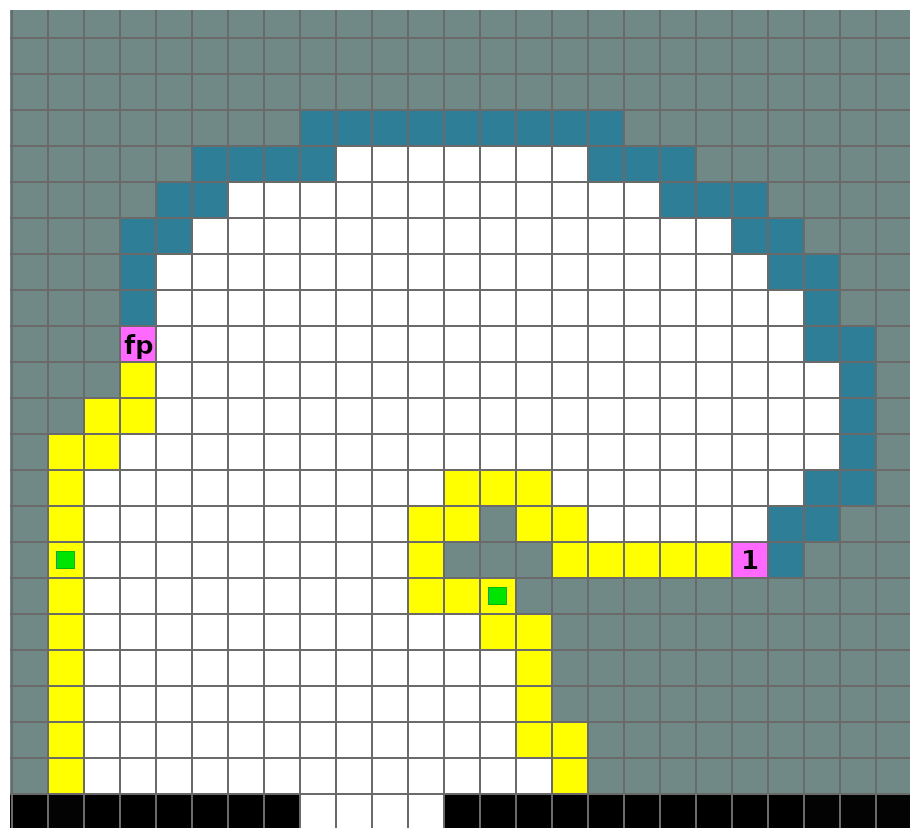
\includegraphics[clip=true, width=0.40\textwidth]{imagenes/ejemploSimpCub/d1.png}}
  \subfloat[Existen celdas más alejadas que $2*rango$, los candidatos se obtienen con $radio=rango$. ]{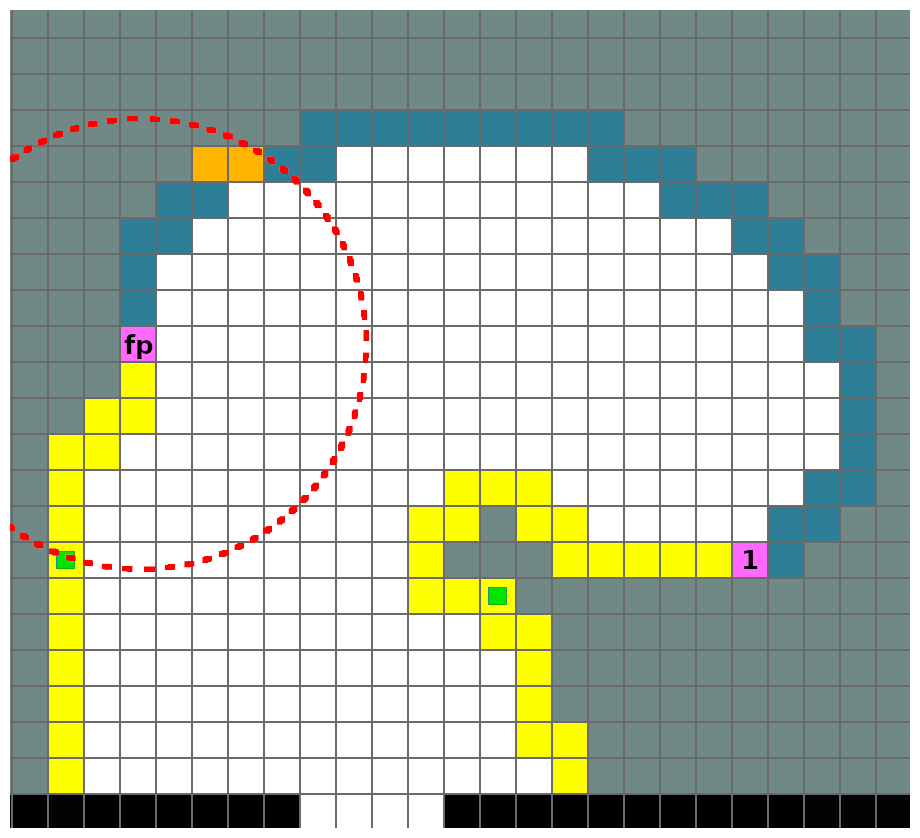
\includegraphics[clip=true, width=0.40\textwidth]{imagenes/ejemploSimpCub/d3.png}}
  \subfloat[Se elige arbitrariamente un candidato como $\mli{fs}$, se actualiza $\mli{UF}$, $\mli{FS_i}$ y $\mli{FP}$.]{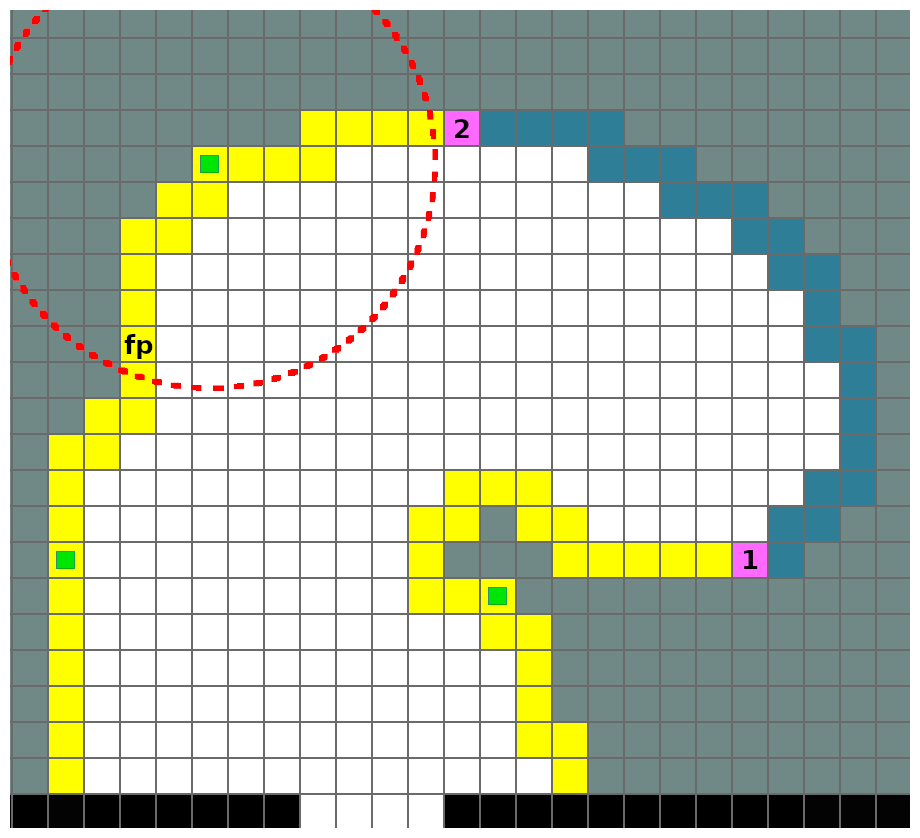
\includegraphics[clip=true, width=0.40\textwidth]{imagenes/ejemploSimpCub/d5.png}}

  \subfloat[Se obtiene $\mli{fp}$ desencolando de $\mli{FP}$.]{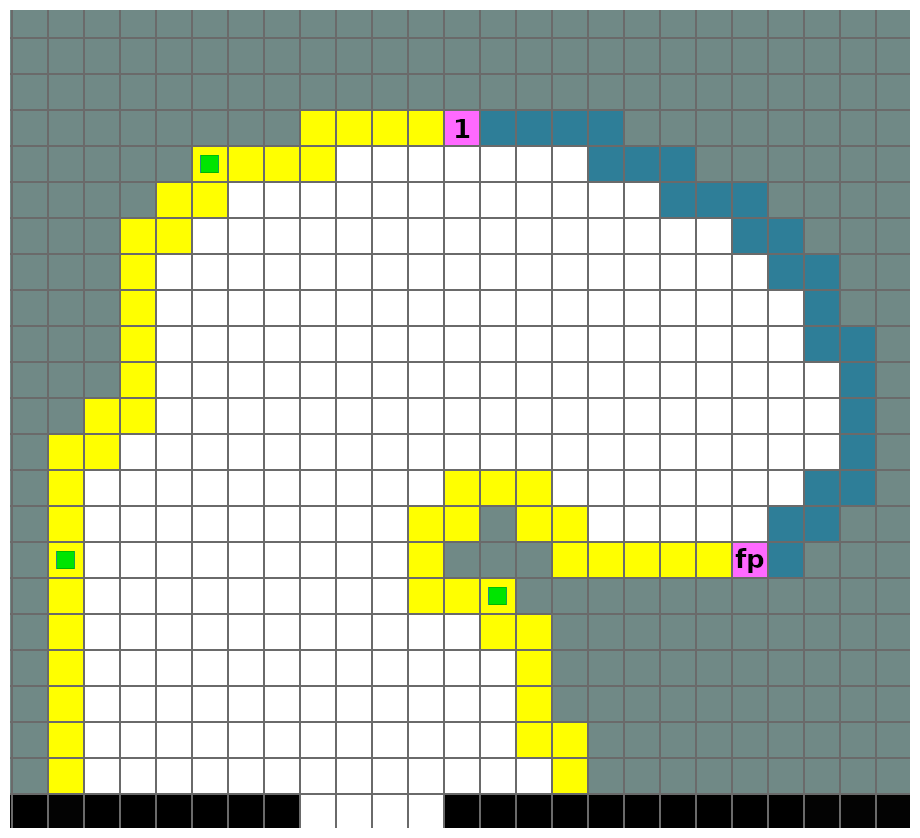
\includegraphics[clip=true, width=0.40\textwidth]{imagenes/ejemploSimpCub/e1.png}}
  \subfloat[Existen celdas más alejadas que $2*rango$, los candidatos se obtienen con $radio=rango$. ]{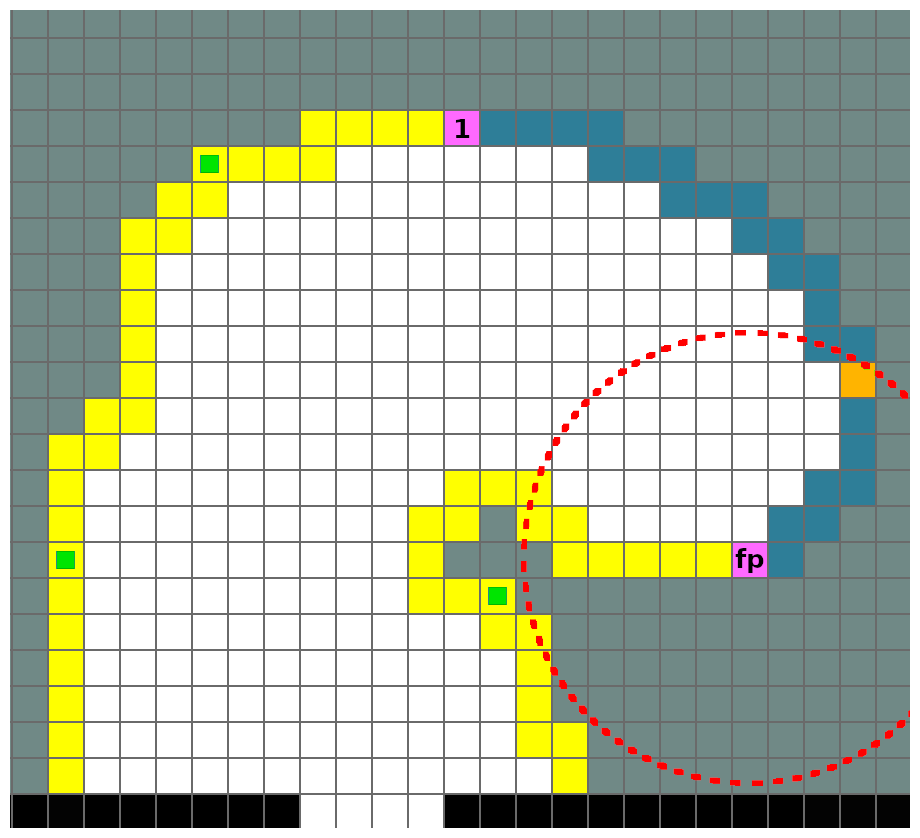
\includegraphics[clip=true, width=0.40\textwidth]{imagenes/ejemploSimpCub/e3.png}}
  \subfloat[Se elige arbitrariamente un candidato como $\mli{fs}$, se actualiza $\mli{UF}$, $\mli{FS_i}$ y $\mli{FP}$.]{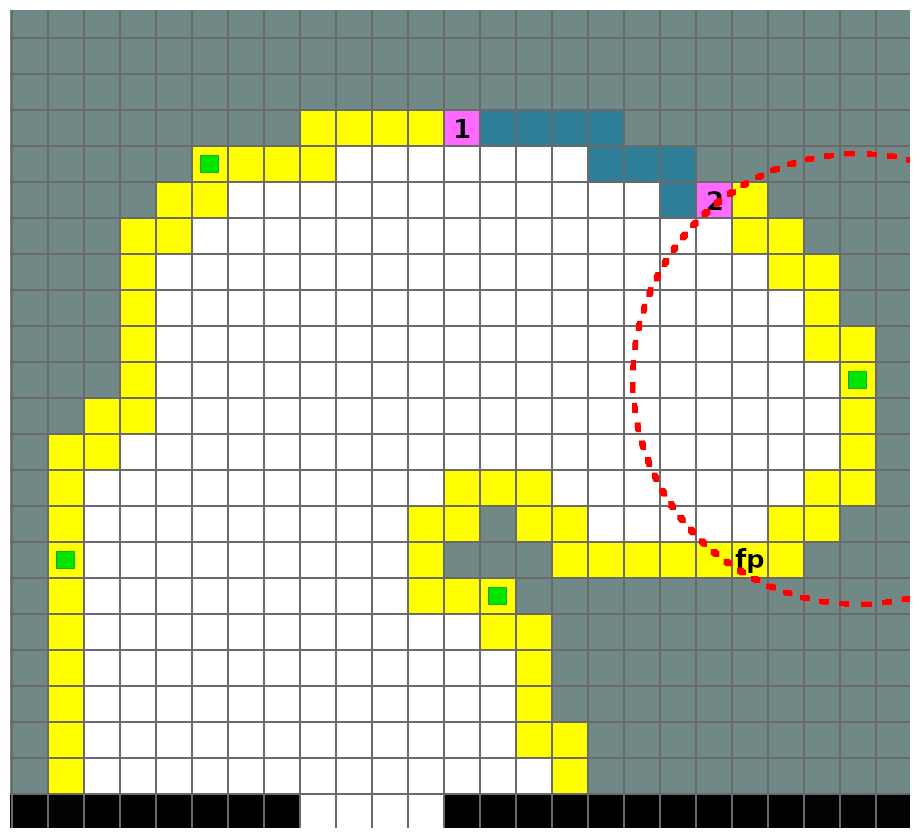
\includegraphics[clip=true, width=0.40\textwidth]{imagenes/ejemploSimpCub/e5.png}}


 \phantomcaption
\end{figure}

\setcounter{figure}{0}

\begin{figure}[H]
  \setcounter{subfigure}{14}
  \centerfloat

  \subfloat[Se obtiene $\mli{fp}$ desencolando de $\mli{FP}$.]{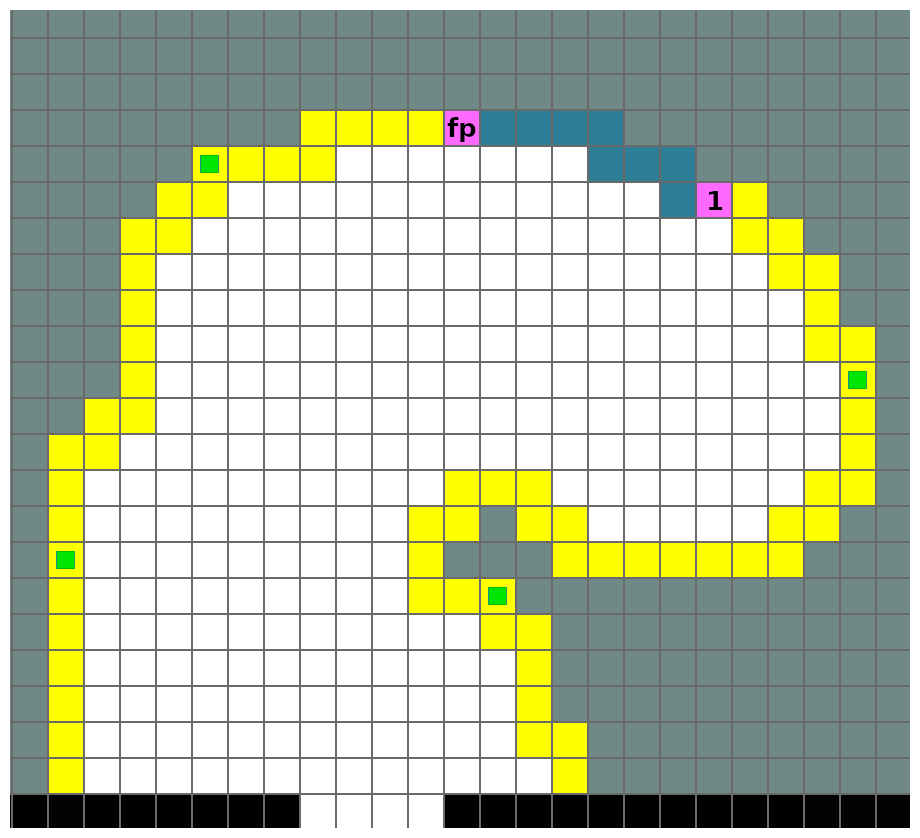
\includegraphics[clip=true, width=0.40\textwidth]{imagenes/ejemploSimpCub/f1.png}}
  \subfloat[No existen celdas más alejadas que $2*rango$, la celda más alejada esta a $\smallsim7.4$ (largos de celda), los candidatos se obtienen con $radio\cong3.7$ (largos de celda). ]{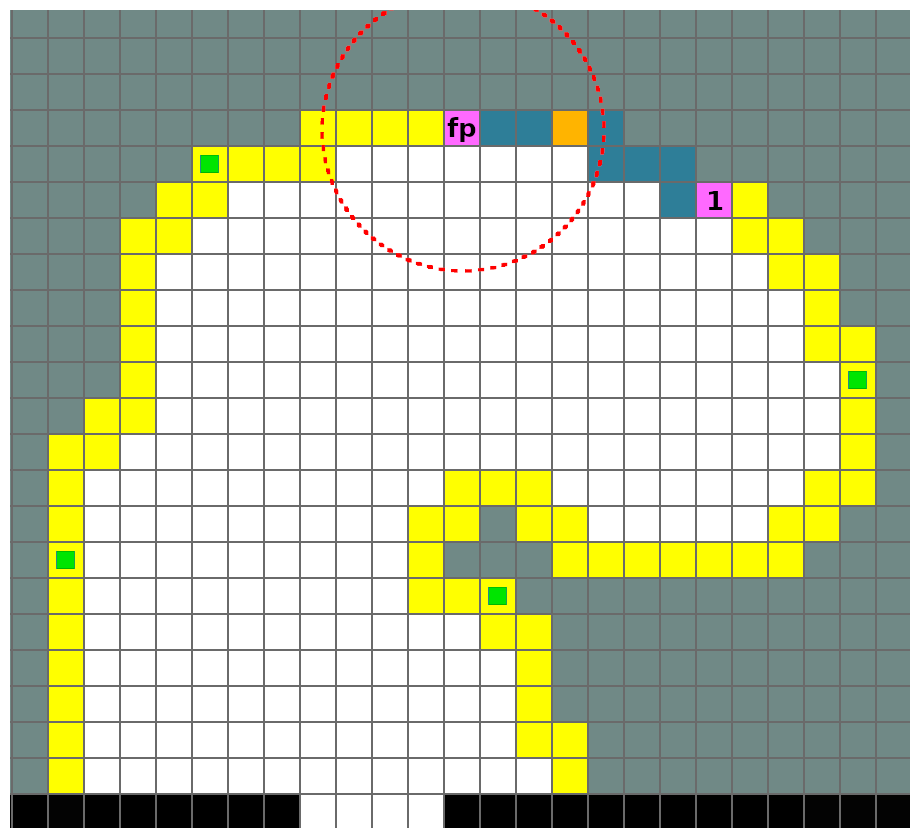
\includegraphics[clip=true, width=0.40\textwidth]{imagenes/ejemploSimpCub/f3.png}}
  \subfloat[Se elige el único candidato como $\mli{fs}$, se actualiza $\mli{UF}$, $\mli{FS_i}$ y $\mli{FP}$.]{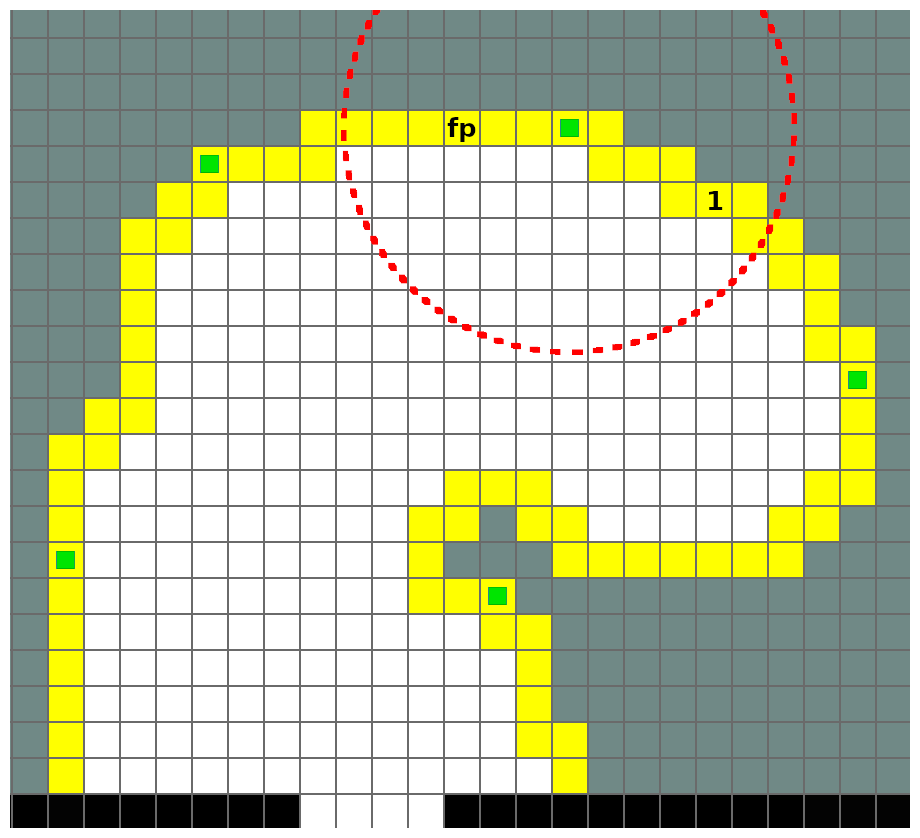
\includegraphics[clip=true, width=0.40\textwidth]{imagenes/ejemploSimpCub/f4.png}}


  \subfloat[$\mli{UF}=\emptyset$ por lo que el algoritmo finaliza.]{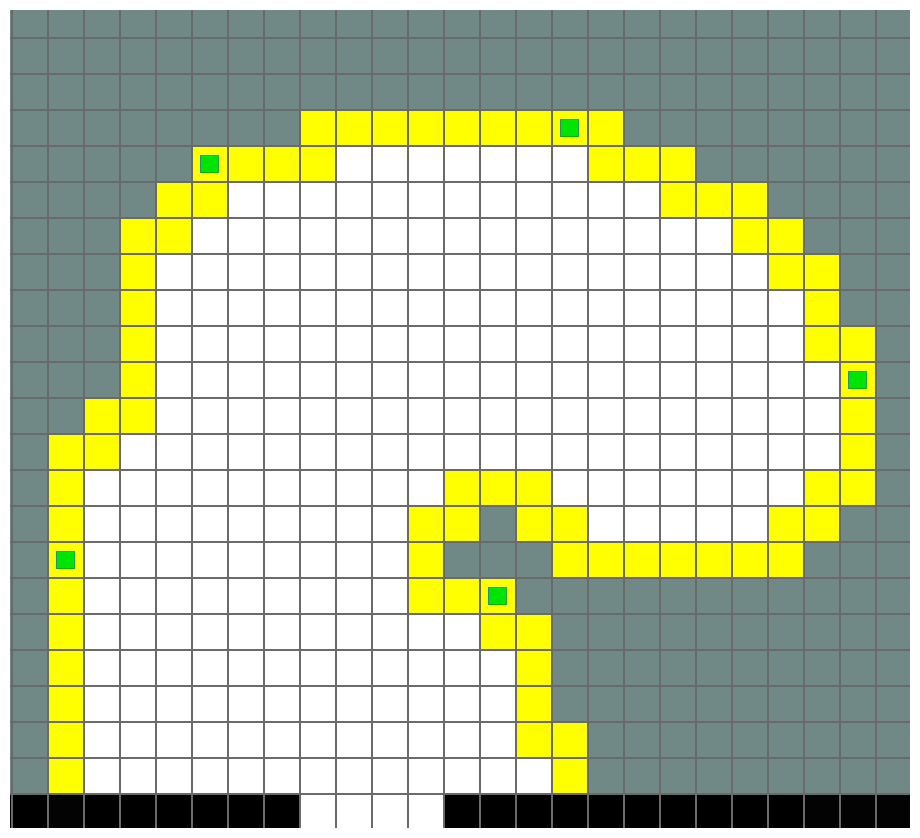
\includegraphics[clip=true, width=0.40\textwidth]{imagenes/ejemploSimpCub/zfinal1.png}}
  % \subfloat[$\mli{UF}=\emptyset$ por lo que el algoritmo finaliza.]{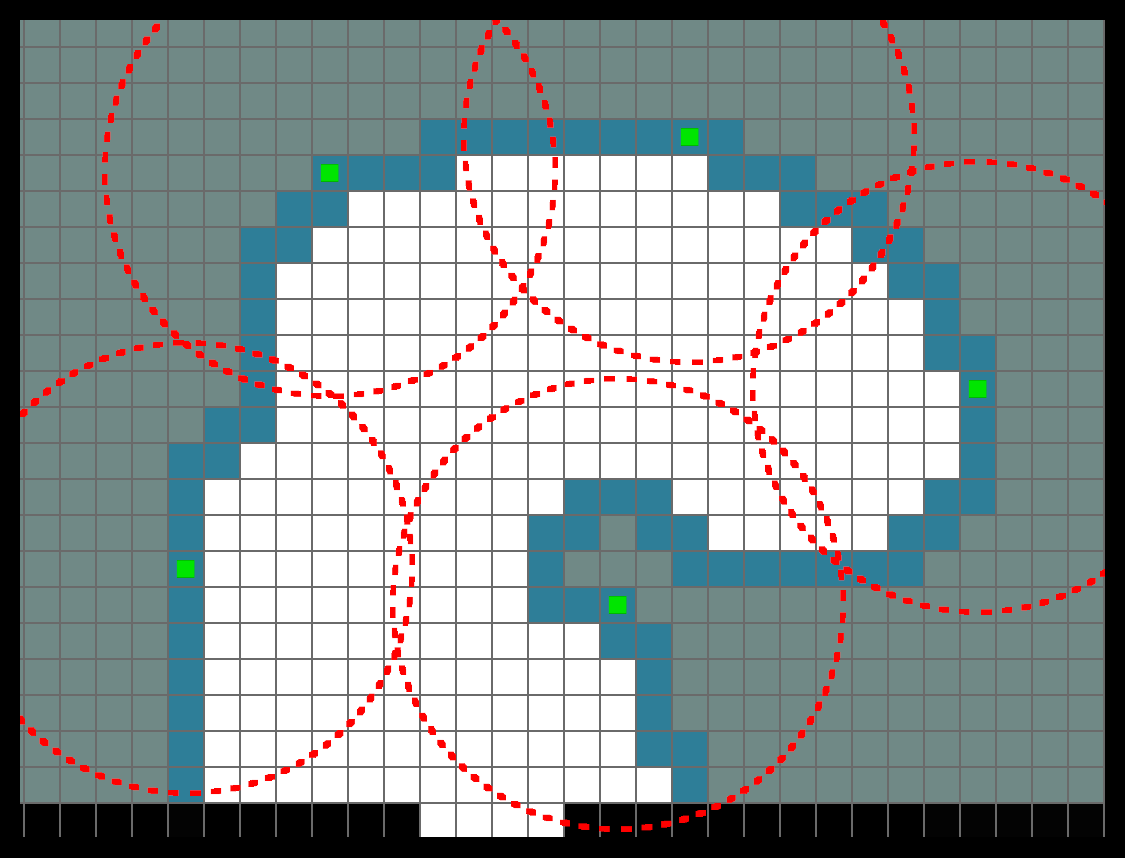
\includegraphics[clip=true, width=0.40\textwidth]{imagenes/ejemploSimpCub/zfinal3.png}}

  \caption[Proceso de simplificación de fronteras según cubrimiento.]{Proceso
    de simplificación de fronteras según cubrimiento. Las fronteras de $F_i$ se
    indican con azul si pertenecen a $\mli{UF}$ y con amarillo de lo contrario.
    Con magenta se indican las celdas en $\mli{FP}$ siendo la numeración su
    orden en la cola y $\mli{fp}$ la ultima desencolada. Las
    circunferencias rojas centradas en $\mli{fp}$ tienen como radio la distancia
    utilizada para obtener los candidatos $\mli{FSC}$ los cuales se indican con
    naranja. Las fronteras significativas se indican con verde, siendo las
    circunferencias rojas de radio $rango=5.6$ (largos de celda) centradas en estas indicadores de su
  cubrimiento.}\label{fig:ejemploFSCubComp}

\end{figure}
